$subject$=Математическая статистика
$teacher$=Лекции Блаженова А. В.
$date$=15.04.2025

\section{Лекция 10.}

\subsection{Свойство ковариации}

\Mem Ковариацией случайных величин $X$ и $Y$ называется величина $\cov (X, Y) = E((X - EX)(Y - EY)) = E(XY) - EX \cdot EY$

Ковариация является индикатором наличия направления связи между двумя случайными величинами

Пусть имеется $(X_1, Y_1), \dots, (X_n, Y_n)$ случайных величин $X$ и $Y$

\Def Выборочной ковариацией называется величина $\samplecov (X, Y) = \overline{xy} - \overline{x} \cdot \overline{y}$

По Закону Больших Чисел ясно, что $\samplecov (X, Y) \longrightarrow \cov (X, Y)$, поэтому выборочная ковариация является оценкой

\begin{MyTheorem}
    \Ths Выборочная ковариация является точечной состоятельной, но смещенной оценкой ковариации. 
    Несмещенной оценкой будет $\frac{n}{n - 1} \samplecov (X, Y)$
\end{MyTheorem}

Ковариация и выборочная ковариация обладают свойствами

\begin{enumerate}
    \item $\cov (X, Y) = \cov (Y, X)$
    \item $\cov (X, a) = 0$, где $a = \const$
    \item $\cov (X, bY) = b \cov (X, Y)$
    \item $\cov (X + Y, Z) = \cov (X, Z) + \cov (Y, Z)$
    \item $\cov (X, X) = D(X), \samplecov (X, X) = D^* (X)$
    \item $D(X + Y) = DX + DY + 2\cov (X, Y)$
\end{enumerate}

\Nota В дальнейшем под $\cov (X, Y)$ будет пониматься выборочная ковариация

\hypertarget{linear_regression_hypothesis}{}

\subsection{Анализ модели линейной парной регрессии}

Пусть при $n$ экспериментах получены значения случайных величин $X$ и $Z$: $(X_1, Z_1), \dots, (X_n, Z_n)$

Пусть $X = \alpha + \beta Z + \varepsilon$ - теоретическая модель линейной регрессии, где $\varepsilon$ - случайная величина,
отражающая влияние невключенных факторов, нелинейность модели, ошибок измерений и просто случая.

Пусть построили с помощью метода наименьших квадратов выборочное уравнение линейной регрессии $\hat X = a + b Z$

Обозначим $\hat \varepsilon_i = X_i - \hat X_i$ - экспериментальная ошибка, разница между наблюдаемыми значениями и 
вычисляемыми по модели

Тогда $X_i = \hat X_i + \hat \varepsilon_i$ или $X_i = a + b Z_i + \hat \varepsilon_i$, где $a$ и $b$ - точечные оценки параметров $\alpha$ и $\beta$

Свойства $\hat \varepsilon_i$:

\begin{enumerate}
    \item $\overline{\hat \varepsilon_i} = 0$

    \begin{MyProof}
        $a = \overline{X} - b \overline{Z} \Longrightarrow a + b \overline{Z} = \overline{X} \Longrightarrow \overline{\hat \varepsilon_i} = \overline{X_i - (a + b Z_i)} = \overline{X} - \overline{a + b Z_i} = \overline{X} - \overline{X} = 0$
    \end{MyProof}

    \item $\cov (\hat X, \hat \varepsilon) = 0$

    \begin{MyProof}
        $b = \overline{\overline{xz} - \overline{x} \cdot \overline{z}}{\hat \sigma^2_z} = \overline{\cov (X, Z)}{D(Z)} \Longrightarrow \cov (X, Z) - b D(Z) = 0$

        $\cov (\hat X, \hat \varepsilon) = \cov (a + b Z, X - a - bZ) = \cov (bZ, X - bZ) = \cov (bZ, x) - \cov (bZ, bZ) = b \cov (Z, X) - b^2 D(Z) = b (\cov (Z, X) - b D(Z)) = 0$
    \end{MyProof}
\end{enumerate}

\subsection{Анализ дисперсии результата}

\Def $D(X) = \frac{1}{n} \sum_{i = 1}^n (X_i - \overline{X})^2$ - дисперсия наблюдаемых значений

\Defs $\hat D(X) = \frac{1}{n} \sum_{i = 1}^n (\hat X_i - \overline{X})^2$ - дисперсия расчетных значений

\Defs $D(\hat \varepsilon) = \frac{1}{n} \sum_{i = 1}^n (\hat \varepsilon_i)^2$ - дисперсия остатков

Так как $X = \hat X + \hat \varepsilon$, $\cov (\hat X, \hat \varepsilon) = 0$, то $D(X) = D(\hat X) + D(\hat \varepsilon) + 2\cov (\hat X, \hat \varepsilon) = D(\hat X) + D(\hat \varepsilon)$

\begin{MyTheorem}
    \Ths $D(X) = D(\hat X) + D(\hat \varepsilon)$
\end{MyTheorem}

Очевидно, что качество модели будет тем лучше, чем меньше будет дисперсия остатков

\Def Коэффициентом детерминации $R^2$ называется величина $R^2 = \frac{D(\hat X)}{D(X)}$ или $R^2 = 1 - \frac{D(\hat \varepsilon)}{D(X)}$

\Notas Смысл $R^2$ - доля объясненной дисперсии, а $1 - R^2$ - доля необъясненной дисперсии

Свойства: 

\begin{enumerate}
    \item $0 \leq R^2 \leq 1$
    \item Если $R^2 = 1$, то $D(\hat \varepsilon) = 0 \Longrightarrow \hat \varepsilon_i = \overline{\hat \varepsilon_i} = 0$, то есть точки лежат строго на 
    линии регрессии, модель идеальна

    \item Если $R^2 = 0$, то $D(\hat X) = 0 \Longrightarrow \hat X = \overline{x}$, то есть получаем примитивную, ничего не объясняющую модель
\end{enumerate}

Чем больше $R^2$, тем лучше качество модели

\subsection{Проверка гипотезы о значимости уравнения регрессии}

Проверяется $H_0 : R^2_\text{теор} = 0$ (уравнение регрессии статистически не значимо) против $H_1 : R^2_\text{теор} \neq 0$

\begin{MyTheorem}
    \Ths Если $H_0$ верна, то $F = \frac{R^2 (n - 2)}{1 - R^2} \in F(1, n - 2)$
\end{MyTheorem}

Пусть $t_\alpha$ - квантиль $F(1, n - 2)$ уровня $\alpha$, тогда:

\begin{cases}
    H_0 : R^2_{\text{теор}} = 0 & \text{ если } F < t_\alpha \\
    H_0 : R^2_{\text{теор}} \neq 0 & \text{ если } F \geq t_\alpha \\
\end{cases}

\Nota Если $H_0 : R^2_{\text{теор}} = 0$, то $H_0 : \beta = 0$

\hypertarget{correlation_coefficient_connection}{}

\subsection{Связь между коэффициентом детерминации и коэффициентом линейной корреляции}

\begin{enumerate}
    \item $\sqrt{R^2} = r_{\hat X, X}$ - коэффициент корреляции между $\hat X$ и $X$
    \begin{MyProof}
        $r_{\hat X, X} = \frac{\cov (\hat X, X)}{\sqrt{D(\hat X) D(X)}} = \frac{\cov (\hat X, \hat X + \hat \varepsilon)}{\sqrt{D(\hat X) D(X)}} = 
        \frac{D(\hat X) + \cancelto{0}{\cov (\hat X, \hat \varepsilon)}}{\sqrt{D(\hat X) D(X)}} = \sqrt{\frac{D(\hat X)}{D(X)}} = R$
    \end{MyProof}

    \item $r_{\hat X, X} = |r_{X, Z}|$

    \begin{MyProof}
        $\cov (\hat X, X) = \cov (a + bZ, X) = b \cov (Z, X)$

        $D(\hat X) = D(a + b Z) = b^2 D(Z)$

        $r_{\hat X, X} = \frac{\cov (\hat X, X)}{\sqrt{D(\hat X) D(X)}} = \frac{b \cov (Z, X)}{\sqrt{b^2 D(Z) D(X)}} = \left|\frac{\cov (X, Z)}{\sqrt{D(Z) D(X)}}\right| = |r_{X, Z}|$
    \end{MyProof}
\end{enumerate}

Следствие 1: в случае линейной парной регрессии коэффициент детерминации равен квадрату коэффициенту корреляции

Следствие 2: в случае линейной парной регрессии совпадают результаты проверки гипотез 
$H_0 : R^2_{\text{теор}} = 0 \Longleftrightarrow H_0 : r = 0 \Longleftrightarrow H_0 : \beta = 0$

\subsection{Теорема Гаусса-Маркова}

\hypertarget{gauss_markov_theorem}{}

\begin{MyTheorem}
    \Ths Пусть $X_i = \alpha + \beta Z_i + \varepsilon_i$ - теоретическая модель регрессии

    $X = a + b Z$ - модель, полученная по методу наименьших квадратов

    Если выполнено условия:

    \begin{enumerate}[label=\asbuk*),ref=\asbuk*]
        \item Случайные члены $\varepsilon_i$ независимые случайные величины, имеющие одинаковое нормальное распределение $\varepsilon_i \in N(0, \sigma^2)$
        \item Случайные величины $\varepsilon_i$ и $Z_i$ - независимы
    \end{enumerate}

    Тогда $a$ и $b$ - состоятельные, несмещенные, эффективные оценки параметров $\alpha$ и $\beta$, то есть

    \begin{enumerate}
        \item Состоятельность: $a \underset{n \to \infty}{\ConvergesInProbability} \alpha, b \underset{n \to \infty}{\ConvergesInProbability} \beta$
        \item Несмещенность: $Ea = \alpha, Eb = \beta$
        \item Наименьшая дисперсия, равная:

        $D a = \frac{\overline{z^2} \sigma^2}{n D(Z)}, Db = \frac{\sigma^2}{n D(Z)}$
    \end{enumerate}
\end{MyTheorem}

\Nota Если не выполняется условие а), то есть ошибки зависимы или имеют разную дисперсию, то оценки становятся неэффективными. 
Если не выполнено условие б), то оценки становятся смещенными и несостоятельными

\subsection{Стандартные ошибки коэффициентов регрессии}

\hypertarget{regression_coefficient_error}{}

Из теоремы видим, что $Da$ и $Db$ зависят от дисперсии $\sigma^2$ случайного члена. 
По экспериментальным ошибкам получаем оценку данной дисперсии:

$D(\hat \varepsilon) = \frac{1}{n} \sum_{i = 1}^n {\hat \varepsilon_i}^2 \underset{n \to \infty}{\ConvergesInProbability} \sigma^2$

Однако эта оценка является смещенной:

$E(D(\hat \varepsilon)) = \frac{n - 2}{n} \sigma^2$

Поэтому несмещенной оценкой дисперсии $\sigma^2$ является величина $S^2 = \frac{1}{n - 2} \sum_{i = 1}^n {\hat \varepsilon_i}^2$

\Def Величина $S$ называется стандартной ошибкой регрессии

Смысл: характеризует разброс наблюдаемых значений вокруг линии регрессии

\Nota Заменим в теореме Гаусса-Маркова $\sigma^2$ на $S^2$, получаем оценки дисперсий $Da$ и $Db$: $S_a^2 = \frac{\overline{z^2} S^2}{n D(z)}, S^2_b = \frac{S^2}{n D(Z)}$

\Def $S_a$ и $S_b$ называются стандартным ошибками коэффициентов регрессии

\subsection{Прогнозирование регрессионных моделей}

Пусть $X = \alpha + \beta Z + \varepsilon$ - теоретическая модель

$\hat X = a + b Z$ - модель МНК, построенная по выборке объема $n$

С помощью данной модели надо дать прогноз значения $X_p$ при заданном значении $Z_p$ и оценить качество прогноза 

Теоретическое значение - $X_p = \alpha + \beta Z_p + \varepsilon$, а точечный прогноз $\hat X_p = a + b Z_p$

Разность между ними $\Delta_p = \hat X_p - X_p$ называется ошибкой предсказания

Свойства $\Delta_p$:

\begin{enumerate}
    \item $E \Delta_p = 0$
    \item $D (\Delta_p) = \left(1 + \frac{1}{n} + \frac{(Z_p - \overline{z})^2}{n DZ}\right) \sigma^2$

    Заменив $\sigma^2$ на $S^2$, получим стандартную ошибку прогноза: $S_{\Delta_p} = S \sqrt{1 + \frac{1}{n} + \frac{(Z_p - \overline{z})^2}{n DZ}}$

    \item $D(\Delta_p) > \sigma^2$ - то есть точность прогноза ограничена случайным членом $\varepsilon$

    \item При $n \to \infty$ $D(\Delta_p) \ConvergesInProbability \sigma^2$ - качество модели тем лучше, чем больше объем выборки

    \item Чем больше $Z_p$ отклоняется от $\overline{z}$, тем хуже качество прогноза. Наилучшее качество в точке $Z_p = \overline{z}: \ D(\Delta_p) = \left(1 + \frac{1}{n}\right) \sigma^2$

    % https://www.geogebra.org/calculator/brxkjkqc

    \begin{center}
        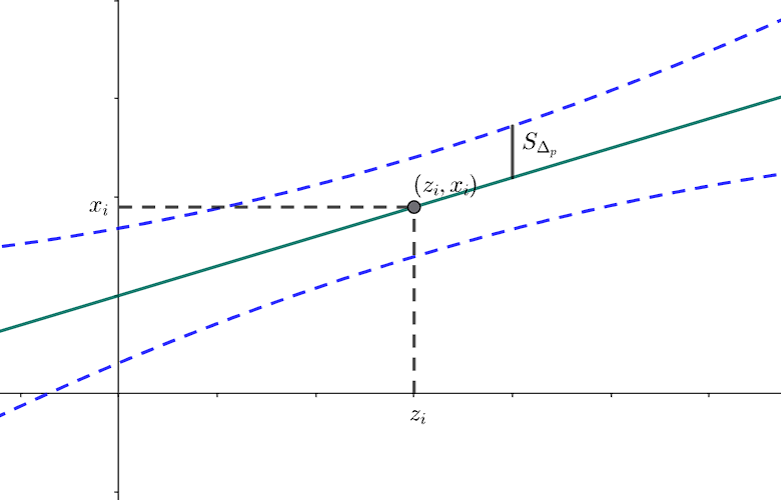
\includegraphics[width=10cm]{mathstat/images/mathstat_2025_04_15_1}
    \end{center}
\end{enumerate}

\subsection{Доверительные интервалы прогноза и коэффициентов уравнения линейной регрессии}

Пусть $t_\gamma$ - квантиль $|T_{n - 2}|$ уровня $\gamma$

Тогда доверительные интервалы надежности $\gamma$ для параметров $\alpha$ и $\beta$:

$\qquad \alpha: (a - t_\gamma S_a; a + t_\gamma S_a)$

$\qquad \beta: (b - t_\gamma S_b; b + t_\gamma S_b)$

Доверительный интервал для прогноза $X_p: (\hat X_p - t_\gamma S_{\Delta_p}; \hat X_p + t_\gamma S_{\Delta_p})$

